\documentclass[UTF8]{ctexart}
\usepackage[a4paper,left=3cm,right=3cm,top=2cm]{geometry}
\usepackage{amsmath}
\usepackage{enumitem}
\usepackage{float}
\usepackage{threeparttable}
\usepackage{caption}
\usepackage{multirow}
\usepackage{graphicx}
\usepackage{listings}
\usepackage{xcolor}
\usepackage{amssymb}
\renewcommand{\figurename}{Figure}
\definecolor{dkgreen}{rgb}{0,0.6,0}
\definecolor{gray}{rgb}{0.5,0.5,0.5}
\definecolor{mauve}{rgb}{0.58,0,0.82}
\lstdefinelanguage{LC3}{
  morekeywords={ADD, AND, BR, BRn, BRnz, BRnzp, BRnp, BRz, BRzp, BRp, JMP, JSR, LD, LDI, LDR, LEA, NOT, ST, STI, STR},
  sensitive=false,
  morecomment=[l]{;},
  morestring=[b]",
  morekeywords=[2]{R0, R1, R2, R3, R4, R5, R6, R7}, % Define register keywords
}
\lstset{frame=tb,
  language=LC3,
  aboveskip=3mm,
  belowskip=3mm,
  showstringspaces=false,
  columns=flexible,
  basicstyle={\small\ttfamily},
  numbers=left,%设置行号位置none不显示行号
  numberstyle=\tiny\courier, %设置行号大小
  numberstyle=\tiny\color{gray},
  keywordstyle=\color{blue},
  keywordstyle=[2]\color{purple},
  commentstyle=\color{dkgreen},
  stringstyle=\color{mauve},
  breaklines=true,
  breakatwhitespace=true,
  escapeinside=`,%逃逸字符(1左面的键),用于显示中文例如在代码中`中文...`
  tabsize=4,
  extendedchars=false %解决代码跨页时,章节标题,页眉等汉字不显示的问题
}

\setlength\lineskiplimit{5.25bp}
\setlength\lineskip{5.25bp}

\title{Lab 4 Report}
\author{崔士强 PB22151743}
\date{December 17, 2023}

\bibliographystyle{plain}

\begin{document}

\maketitle
\section{Purpose}
\subsection{Problem description}
The purpose of the program is to compute the number of steps required to
unlock Baguenaudier, a series of rings fitted on a board. A ring can be put on or removed if one of the two conditions below is met:
\begin{enumerate}
  \item It is the 1st ring.
  \item It is the $i$-th ring, and the $(i-1)$-th ring is on the board, but the first $(i-2)$ rings are not on the board.
\end{enumerate}

The state of rings are represented by a n-bit binary number. 1 means the corresponding ring is removed from the board. 
\subsection{Anticipated outcomes}
The state after each operation will be stored in memory locations starting from \lstinline{x3101}.

\section{Principles}
\subsection{Overview}
The problem can be recursively solved. Let operations of removing n rings be denoted as $R(n)$, 
and the operations of putting on n rings as $P(n)$. Thus we have:
\begin{equation}
  P(i)=
  \begin{cases}
    Nothing\ to\ do,& n=0 \\
    Put\ the\ 1^{st}\ ring,& n=1 \\
    P(i-1)+R(i-2)+Put\ the\ i^{th}\ ring+P(i-2),& n\geq  2
  \end{cases}
\end{equation}
\begin{equation}
  R(i)=
  \begin{cases}
    Nothing\ to\ do,& n=0 \\
    Remove\ the\ 1^{st}\ ring,& n=1 \\
    R(i-2)+Remove\ the\ i^{th}\ ring+P(i-2)+R(i-1),& n\geq  2 
  \end{cases}
\end{equation}
So the general idea is to use two subroutines to implement $P(n)$ and $R(n)$, and call the 
subroutines within subroutines.
\subsection{Stack}
Due to the fact that the subroutines are repeatedly called, the data in relevant
registers may be lost(e.g. R7). Solution is to use a stack. When a subroutine is called,
data in registers are pushed onto the stack first. Before returning, the data is poped back.
In this program, R6 is the stack pointer which is initialized with \lstinline{x4000}. 

Example of operations on the stack:
\begin{lstlisting}
                ADD     R6, R6, #-1
                STR     R0, R6, #0      ; Push R0 onto stack
                LDR     R0, R6, #0      ; Pop R0 back
                ADD     R6, R6, #1
\end{lstlisting}
\subsection{Operations on the i-th ring}
Suppose we have R5 stored a 16-bit binary number with only the i-th bit set as 1, performing 
bit-wise OR with the number representing current state gives the result after removing
the i-th ring.

According to DeMorgan Rule:
\[A\ OR\ B = \overline{\overline{A}\ AND\ \overline{B}}\]
OR can be implemented by \lstinline{AND} and \lstinline{NOT} instructions:
\begin{lstlisting}
                NOT     R1, R1
                NOT     R5, R5
                AND     R1, R1, R5
                NOT     R1, R1
                ADD     R3, R3, #1
                STR     R1, R3, #0      ; Remove the i-th ring
\end{lstlisting}

And performing bit-wise NAND will give the result after putting the i-th ring:
\begin{lstlisting}
                NOT     R5, R5
                AND     R1, R1, R5      
                ADD     R3, R3, #1
                STR     R1, R3, #0      ; Put the i-th ring
\end{lstlisting}

In order to get the right number in R5, we use a subroutine to repeatedly move the number 1 left:
\begin{lstlisting}
SINGLEBIT       ADD     R6, R6, #-1
                STR     R0, R6, #0      ; Push R0 onto stack
                
                ADD     R0, R0, #-1
                AND     R5, R5, #0      ; Clear R5
                ADD     R5, R5, #1      ; Set R5 as 1
  
MOVE_LEFT       ADD     R5, R5, R5      ; Multiply R5 by 2
                ADD     R0, R0, #-1
                BRp     MOVE_LEFT
                
                LDR     R0, R6, #0      ; Pop R0 back
                ADD     R6, R6, #1
  RET
\end{lstlisting}
\section{Procedure}
\subsection{Bugs encountered}
\begin{enumerate}
  \item When testing the program, an endless loop is detected. The reason is that in REMOVE subroutine,
  I used AND to remove the i-th bit, while the right way is to use OR.
  \item Another bug comes from misusing of the stack. When pushing a new item onto the stack,
   stack pointer substracts 1, which is \lstinline{ADD R6, R6, #-1}. But I used \lstinline{ADD R6, R6, #1}
   which caused a bug.
\end{enumerate}

\subsection{Chanllenges}
A major chanllenge in the task is the use of subroutines and stack. To get things work properly, 
we need to find out which registers are expected to remain unchanged after calling the subroutine and which are not.

In this case, R0(stores number of rings to be moved) and R7(stores return linkage) are expected to remain unchanged.
So we push R6 and R0 at the beginning of the subroutine, and pop into R0 and R6 before returning.
\clearpage
\section{Results}
Results are shown below:
\begin{figure}[h]
        \centering
        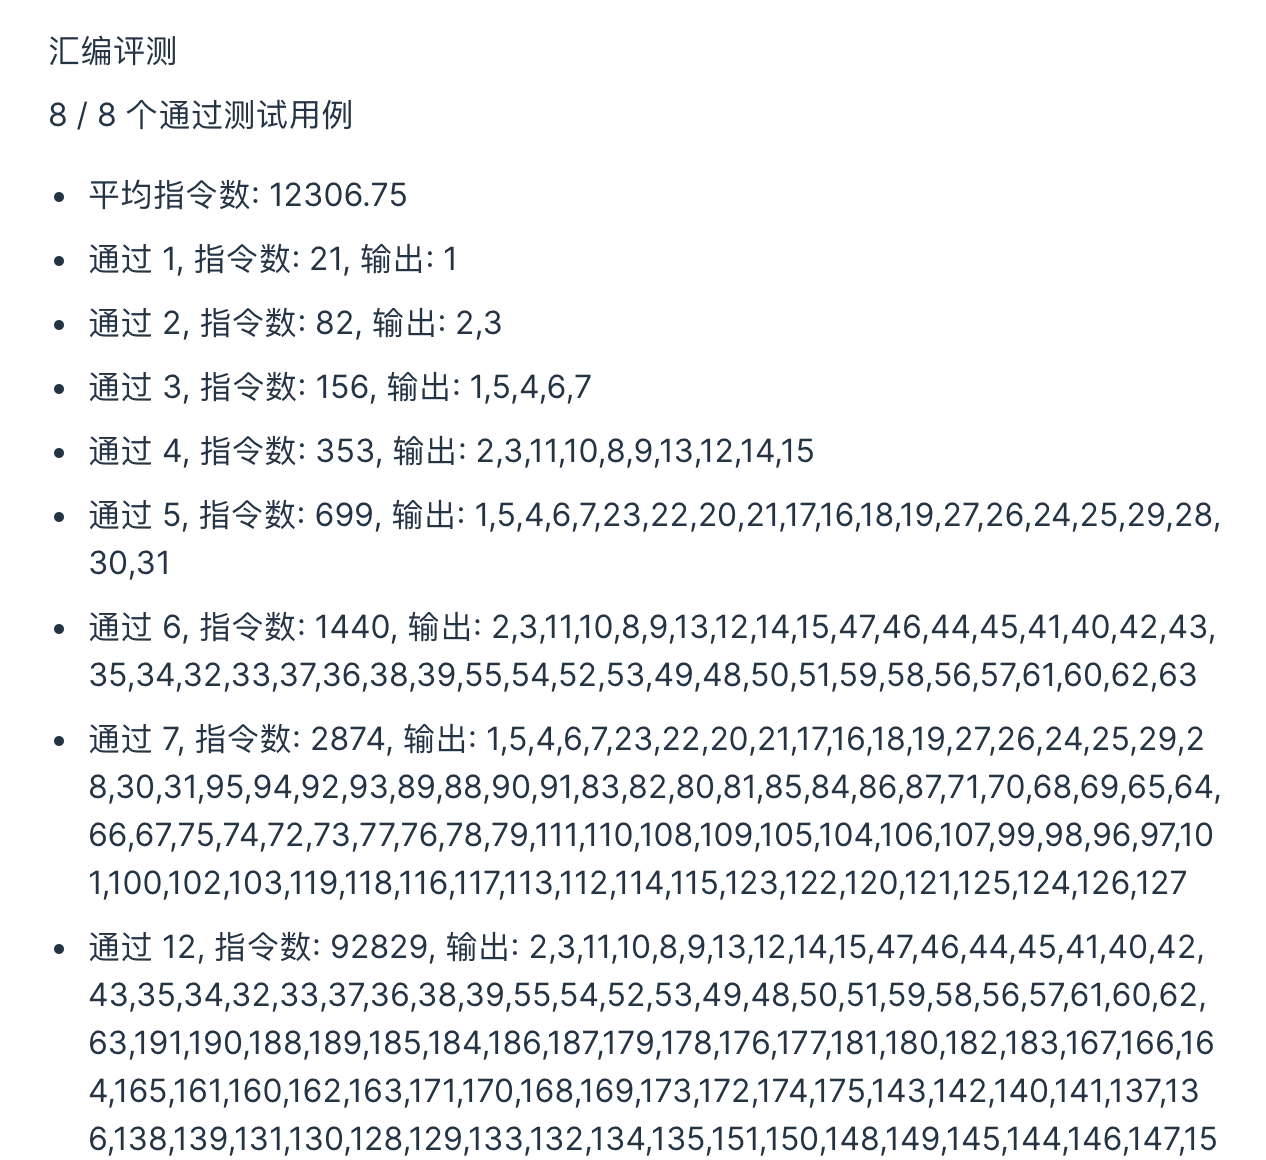
\includegraphics[scale=0.5]{result.png}
        \caption{Result}
\end{figure}

\bibliography{math}

\end{document}
\iffalse
\begin{figure}[H]
    \centering
    \includegraphics[scale=0.5]{name.png}
    \caption{name}
\end{figure}
\fi
